\documentclass[compress,xcolor={dvipsnames}]{beamer}
\usepackage{fancyvrb,newverbs} % For customized verbatim
\usepackage{calligra} % A fancy text for ending `Thank you'
\usepackage[T1]{fontenc}
\usefonttheme[onlymath]{serif}

\author{Zihang Wang}
\title{Phase Field Tutorial}
\subtitle{C++ Programming and Calculation Examples}
\institute{Central South University}

\AtBeginSubsection[]
{
	\begin{frame}
		\tableofcontents[sectionstyle=show/shaded,subsectionstyle=show/shaded/hide,subsubsectionstyle=show/shaded/hide]
	\end{frame}
}
\usetheme{Berlin}

\setbeamertemplate{footline} {
    \begin{beamercolorbox}[ht=2.5ex,dp=1.125ex,
      leftskip=.3cm,rightskip=.3cm plus1fil]{title in head/foot}
      {\usebeamerfont{institute in head/foot}\usebeamercolor[fg]{institute in head/foot}\insertshortinstitute}
      \hfill
      {\centering\usebeamerfont{title in head/foot}\insertshortsubtitle}
      \hfill
      {\usebeamerfont{frame number}\usebeamercolor[fg]{frame number}\insertframenumber~/~\inserttotalframenumber}
    \end{beamercolorbox}
    \begin{beamercolorbox}[colsep=1.5pt]{lower separation line foot}
    \end{beamercolorbox}
}

% ---------------------------------------------------------------------------
\definecolor{cverbbg}{gray}{0.93}

\newenvironment{cverbatim}
 {\SaveVerbatim{cverb}}
 {\endSaveVerbatim
  \flushleft\fboxrule=0pt\fboxsep=.5em
  \colorbox{cverbbg}{\BUseVerbatim{cverb}}%
  \endflushleft
}
\newenvironment{lcverbatim}
 {\SaveVerbatim{cverb}}
 {\endSaveVerbatim
  \flushleft\fboxrule=0pt\fboxsep=.5em
  \colorbox{cverbbg}{%
    \makebox[\dimexpr\linewidth-2\fboxsep][l]{\BUseVerbatim{cverb}}%
  }
  \endflushleft
}
\newverbcommand{\cverb}
  {\setbox\verbbox\hbox\bgroup}
  {\egroup\colorbox{cverbbg}{\box\verbbox}}

\setlength{\parindent}{2em}

\newcommand{\bhref}[2]{
    \href{#1}{\color{blue}{#2}}
}
% ---------------------------------------------------------------------------

\begin{document}
\begin{frame}
    \titlepage
    \begin{figure}[!h]
        \centering
        
\includegraphics[width=0.18\linewidth]{pic/csulogo.jpg}
        
\includegraphics[width=0.25\linewidth]{pic/MInDes_Icon.jpg}
    \end{figure}
\end{frame}

\begin{frame}
    \tableofcontents[currentsection, hideothersubsections, sectionstyle=show/show]
\end{frame}

% ---------------------------------------------------------------------------
\section{Review \& Intro}
\begin{frame}
    \frametitle{Quick Review}
    What have we got in the last tutorial?

    \begin{itemize}
        \item Python Installation
        \item Programming Basics (Python)
        \item Forward / Backward Euler Method
        \item OOP and Numerical Integral
        \item OOP and Gradient \& Laplacian
    \end{itemize}

    While, with these numerical methods implemented with Python, Let's try to combine them together, with \emph{C++}.
\end{frame}

\begin{frame}
    \frametitle{C++, a `better C' }
    C++, a programming language designed by Bjarne Stroustrup in 1979, was originally designed to be an improved C, has
    become one of the most popular programming languages in the world. It supports OOP, template programming, and many otehr
    useful features. It's so efficient that can be compared with C. All these features enabling it to be an
    ideal choice for scientific computation.
    \bigbreak
    \pause
    However, it is also a complicated language There are messive details of grammar, and some features
    make it not so friendly to programmers. Some common things in other language could be not that easy in C++.
    \bigbreak
    \pause
    But, fortunately, to learn and do some calculation with C++, all you need is almost there.
\end{frame}

\begin{frame}
    \frametitle{What's our plan?}
    So, where shall we start from? What shall we do? Repeat the algorithm in the last tutorial, and just implement them in C++?
    \bigbreak
    \pause
    That's half-right. We won't cover all details in implementing these algorithm. What we are going to do are:
    \begin{enumerate}
        \item C++ Environment Setup;
        \item C++ Grammar and Features;
        \item Algorithms, again;
        \item Simple Example: 1D Heat Transfer Question.
    \end{enumerate}
    \pause
    That's a lot. Let's start our very first step: environment setup.
\end{frame}

% ---------------------------------------------------------------------------
\section{Setup Your Environment}
\subsection{Before we start}
\begin{frame}
    \frametitle{Make a Choice}
    Okay, you must can't wait to download something. But there are bunch of choices, and some of you might
    end up with wrong configuration, frustrated and stay away from C++ to retain your mental health. So to save your time,
    I recommend three way to get started with C++:
    \pause
    \begin{itemize}
        \item The newest Visual Studio Community Edition if you are runing on Windows.
        \item The GCC compiler tool chain chain with Linux or WSL if you are on Linux or want to give it a try.
        \item The Clang/LLVM compiler tool chain if you are on Mac OS or you just don't like the former two.
    \end{itemize}
    \pause
    Let's see what are they and their features.
\end{frame}
\begin{frame}[fragile]
    \frametitle{VS: The Best IDE for Windows C++ Dev (Maybe\footnote{There are still many other choice, and everyone has their own choice, too. For me myself, VS is good.})}
    Visual Studio (abbr. as \emph{VS}), an IDE from Microsoft for developing C++ or .Net on Windows, usually is the best choice for any C++ programmer
    using Windows. As an IDE, VS is fully equipped with editor, linter, compiler, debugger and analyzer. After some \emph{right} clicks, you are then ready for C++ progrmming, and just skip the tiring prerequisite. You can focus yourself on programming and solving problems.
    \pause

    However, there are flaws in VS. VS is a \emph{BIG} software needing a lot of drive space to install it. And, some components must be installed under your \cverb|C| drive. But if that's okay for you, VS should be the first choice.
\end{frame}

\begin{frame}[fragile]
    \frametitle{GCC: Old, but powerful.}
    Well, if you are not a Windows user, or want to compile C++ for other platform, or just don't want to use VS and MSVC (Compiler used by VS), Then you can try GCC, the GNU Compiler Collection.
    \pause

    What is GNU? GNU is Not Unix! That will be a long story to tell about GNU, Linux, GCC and open source software. But if you are going to write your code on Linux, your first choice will always be GCC tool chain, explicitly, \cverb|g++|, \cverb|gdb| and \cverb|makefile|, which are compiler, debugger and build system, respectively. All of these tools have long histories, but are powerful and never outdated.
    \pause

    If you are interested in GCC and Linux, but already a Windows user, I recommend you to install `WSL' on your Windows. That will give you almost the original experience of a Linux system.
\end{frame}

\begin{frame}
    \frametitle{Clang/LLVM: Progressive New Force}
    If you are on Mac OS, after install gcc and check your installation, you will be surprised by prompt from `Clang'. That's because Mac OS use Clang/LLVM as its default C/C++ compiler.
    \pause

    Clang is a part of LLVM Project, which is originally a research project at University of Illinois. Clang is a compiler that compatible with many backends, such as MSVC and GCC. And, as a fully modularized compiler, it has a great potential to be extended and developed, and is a good example for whom studying compiler theory and language design.
    \pause

    Well, we don't actually need to learn compiler or language design. What's good for choosing Clang? If you are using Mac OS, that will be your first choice. Or you can just give it a try. Clang is famous for its readable and helpful error/warn messages. Maybe you will like it.
\end{frame}
\subsection{Set It Up!}
\begin{frame}[fragile]
    \frametitle{Let's do it}

    By now you should have made your choice. Let's start to set our enviornment up.
    \pause

    If you choose to install Visual Studio from Microsoft, please download the installer (yes, you need install the installer first), and \emph{select `Desktop development with C++'}. Then you can just accept the default settings.
    \pause

    If you choose to install WSL and GNU, I recommend reading WSL guide from Microsoft before install it, and installing VS Code. VS Code has good support to WSL and C++ programming with extension. Then after WSL setup, you can install GNU tool chain by \cverb|sudo apt install build-essential|.
    \pause

    If you are using Mac OS, you can use \cverb|homebrew| to install Clang, and choose your favourite editor or IDE.

\end{frame}

\begin{frame}[fragile]
    \frametitle{Your First C++ Code}

    So, let's try to write a little piece of C++ code.

    Your first C++ code, as usual, will be a simple `Hello World':
    \begin{lcverbatim}
        #include <iostream>

        int main(){
                std::cout<< "Hello C++ World!\n";
            }
    \end{lcverbatim}
    This code includes many points. You use \cverb|#include| to \emph{Copy \& Paste} file \cverb|iostream|, and your program will start executation from the function \cverb|main()|. Finally your code will use \cverb|std::cout| to output a string \cverb|"Hello C++ World"| to your screen, and print a line break using escape character \cverb|'\n'|. Details will be in the next section.

\end{frame}

\begin{frame}[fragile]
    \frametitle{Run it}

    Now, if you are using Visual Studio, you can just click the button: `Local Windows Debugger':
    \begin{figure}[!h]
        \centering
        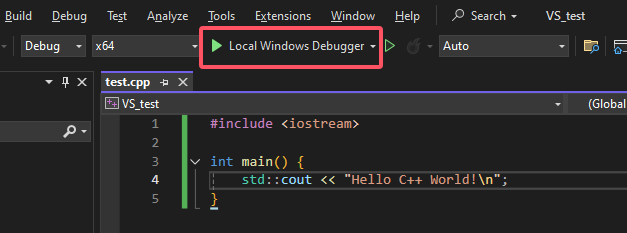
\includegraphics[width=0.50\linewidth]{pic/VS_Build.png}
    \end{figure}
    if you are using Linux or Mac OS, please type \cverb|g++ *.cpp| under the folder your source file locates. You will get a file called \cverb|a.out|. That will be your program and you can run it by typing the followings in your console: \cverb|./a.out|.

    Or, if you are using editor with LSP support, like VSCode, you can just use the extension to run your code.
\end{frame}

\section{C++ Language}
\subsection{Basics about C++}
\begin{frame}[fragile]
    \frametitle{standard libraries, \texttt{\#include} \& \texttt{main}}
    To start with, first we encounter in C++ program is usually several lines looks like \cverb|#include <xxx>|. Here `xxx' is usually one of the \emph{standard libraries}, which are a set of \emph{headers} together with \emph{libraries} that you can use when you want certain functions. For example, if you want to input \& output something, you use \cverb|iostream|; if you want to store something inside a \cverb|vector|, you use \cverb|vector| header.

    Each C++ executable file must contains a \cverb|main| function in its source code. That's where our programs will start to execute from. This might be different from Python (although Python also supports such features, it's not default behaviour).

\end{frame}

\begin{frame}[fragile]
    \frametitle{types and \texttt{std}}
    C++ is a type strict programming language. That's very different from Python: Python is dynamical type language, and value in Python doesn't check the type. While, C++ have statical types, value will have its type by your design, and C++ will check your code about the types before run.

    There are several types you already familar: `int', `float', `bool'(although in C++ both value should be lower case), `char' and so on. You may ask: `Where is `string'?' In C++, we recommend `std' string (although it also supports C-style raw string), which is actually a `class' that you can declare and initialize a `std' string by using \cverb|std::string str = "xxx"|.

    There are also many other `std' things, where `std' is a `namespace' that used by the standard libraries to avoid name conflict.

\end{frame}
\subsection{Flow Control}
\begin{frame}[fragile]
    \frametitle{\texttt{for} loop}

    In C++, flow control such as loop and conditional statements are similar with Python. Here we demonstrate the \cverb|for| loop.

    \cverb|for| loop in C++ start from the key word \cverb|for|, then a parenthesis including three \emph{sentences}: init-declaration, loop condition and an expression that usually increments the loop counter. Then after that, you open a braces and the loop body, for example:

    \begin{lcverbatim}
        for(int i = 0; i < 3; i++){
                std::cout << i << " ";
            }
    \end{lcverbatim}

    This \cverb|for| loop will print \cverb|0 1 2|.

\end{frame}

\begin{frame}[fragile]
    \frametitle{\texttt{if-else} statements}

    Here we introduce the most general conditional statements: \cverb|if else| statements. \cverb|if else| statement in C++ is very similar to that of Python, with only some difference in details:
    \begin{itemize}
        \item Use parenthesis in conditions instead of write out after \cverb|if|;
        \item Use braces to open the body statements instead of open with colon;
        \item Use \cverb|else if| explicitly instead of short-hand form \cverb|elif| in Python
    \end{itemize}
    We don't cover the ternary operator \cverb|?:| and \cverb|switch-case| statements. Feel free to explore them by yourself.

\end{frame}
\subsection{Pointers and Reference}
\begin{frame}[fragile]
    \frametitle{pointers}

    We won't cover too much about the pointer here, but give it a brief introduction. A pointer is a
    special variable that will hold other variable's address (called `points to'). Then you can access the value that this pointer pointing to by dereference the pointer using operator \cverb|*|.

    For example, if you have a variable \cverb|int i = 1| and a pointer \cverb|int *p = &i|, then the pointer \cverb|p| will have the value of the address of \cverb|i|. You can then use \cverb|*p| to get the value of \cverb|i| and change it. As pointer gets the address of that value, the modification on the \cverb|*p| will also be the modification of \cverb|i|.

\end{frame}

\begin{frame}[fragile]
    \frametitle{refernce}

    However, pointer is too low-level that you might find it dangerous and hard to use. In C++, there is another way to do the similar thing but with more friendly grammar: \emph{reference}. For example, to create a reference of \cverb|i| declared before, you use \cverb|int &ref = i|, then \cverb|ref| is the reference of \cverb|i|. You can consider reference is just a nickname, such that you can use this nickname just like the original name.

    The reference and pointer will appear in the \emph{function} part and play a key role.

\end{frame}
\subsection{Function}
\begin{frame}[fragile]
    \frametitle{function}

    Just as Python do, C++ also have \emph{function}, but with slightly different grammar. But here is a good example: the \cverb|main| function. You already have defined the \cverb|main| function for many times, and just like that, you can define another function with the following key pointes:

    \begin{enumerate}
        \item return value type: indicate the what type of the value the function will return
        \item function name: of course the function should have a name (although there is anonymous function called \emph{lambda expression})
        \item function parameter list: Define what parameter type will this function take. You may also set the parameter's tempory name here to use them inside of your function body.
        \item function body: Things that this function will do.
    \end{enumerate}
\end{frame}

\begin{frame}[fragile]
    \frametitle{function: simple example}

    And a typical example will be the \cverb|add| function:
    \begin{lcverbatim}
        double add(double a, double b){
                double c = a+b;
                return c;
            }
    \end{lcverbatim}

    Here, the first \cverb|double| indicates that this function will return a \cverb|double| value; \cverb|add| is this function's name; \cverb|double a| and \cverb|double b| are the function's parameter, indicates this function accpets two \cverb|double| variable as its parameters.

    Then inside the function body, we initialized a new \cverb|double| value \cverb|c| with value \cverb|a+b|, and finally we \cverb|return| the value of \cverb|c|. Notice that we can't access the variable \cverb|c| outside of this function as it's a \emph{local} variable only lives inside of this function.
\end{frame}

\begin{frame}[fragile]
    \frametitle{function parameters and reference}

    Can function change the value of the parameter variable? The answer is: It depends. If you use plain variable as function parameters, the function will \emph{copy} the value of the parameter to the the tempory variables and use these tempory varaibles inside of the function. These tempory variables are local and hence can't be accessed from outside.

    While, if you use reference when you define the parameter list, then when you call the function, the function will not copy the parameter's value, but just use the variables themselves. By this way you can modify the parameters' value inside of the function.

    \emph{Pointer}, originally from C, can also achieve the similar thing. While, as C++ has \emph{reference}, it's much more recommended to use reference instead of pointer.

\end{frame}

\begin{frame}
    \frametitle{Implement algorithms with functions}

    With the language points before, now we shall begin to try implementing the algorithms that we have implemented in Python. That should not be too hard, as we already implemented them once, and this time we won't use OOP paradigm. These algorithms are implemented in form of funtions, such that you can call them directly and easily.

    However, there is still a piece of code that use OOP in C++ to handle the calculation of gradients and laplacians. You can check it out if you like.

\end{frame}

\section{Heat Transfer Simulation}
\subsection{Question statements}
\begin{frame}
    \frametitle{Introduction}

    Now we are going to carry on a simple simulation: heat transfer problem. Although it's not a phase-field simulation, this simulation can still be a good example to demonstrate the basic simulation procedure, which differs from phase-field simulation basically only the underlying theories.

    There is the question: the one-dimensional heat conduction equation without heat source can be expressed as:
    \[
        \rho c_p \frac{\partial T}{\partial t} = \frac{\partial }{\partial x}\left( \lambda\frac{\partial T}{\partial x} \right),
    \]
    where \(\rho\) is density, \(c_p\) is heat capacity, \(\lambda\) is thermal conductivity, \(T\) is the temperature, \(t\) and \(x\) are time and position, respectively.
\end{frame}

\begin{frame}
    \frametitle{Question simplification}

    Here we consider a simplified form, such that the \(\lambda\) is a constant:
    \[
        \frac{\partial T}{\partial t} = \mu \frac{\partial^2 T}{\partial x^2},
    \]
    where \(\mu = \frac{\lambda}{\rho c_p}\). By now we can utilize the tool we have acquired before, such as forward Euler method, finite difference algorithm and so on.

    For this simulation, we shall use the following parameters:

    \begin{center}
        \begin{tabular}{cc}
            \hline
            parameter    & value \\
            \hline
            \(\mu\)      & 1.0   \\
            \(\Delta t\) & 0.2   \\
            \(\Delta x\) & 1     \\
            \hline
        \end{tabular}
    \end{center}
    And we are going to use fixed boundary condition to handle this question.
\end{frame}

\subsection{Programming}
\begin{frame}[fragile]
    \frametitle{Code structure}

    \begin{itemize}
        \item Headers: need \cverb|vector| holding values, \cverb|string| to process strings, \cverb|fstream| to output files, and some other headers to increase usability,
        \item Constants: set the simulation related invariable to constants.
        \item Preprocess: set file output folder, set time counter and so on.
        \item Grid creation and mesh initialization: Assign values to a one-dimension vector according to the position.
        \item Time loop: loop as the time evolution, using forward Euler method.
        \item Mesh loop: iterate each points to calculate their values based on the last time step's result.
        \item File output: Record the result into the files.
        \item Postprocess: Calculate the used time and possible summarization of the program execution.
    \end{itemize}

\end{frame}

\begin{frame}[fragile]
    \frametitle{Code details}

    Here are some details that should be noticed:
    \begin{itemize}
        \item There will be two loops: one for time and another for space; you need to iterate time first and then iterate the space in each time step.
        \item As we are using fixed boundary condition, you have to assign each boundary the fixed value every time step.
        \item The result for the next step should be stored inside a tempory vector, such that the next step's result won't affect this step's calculation.
        \item To obtain the result of 0 step and 600 step, for example, you should set the time loop condition to \cverb|istep < 600+1| to make sure that \cverb|istep| can take 600.
        \item When operate the file io, one should make sure that the file is actually existed / opened.
    \end{itemize}

\end{frame}

\subsection{Results}

\begin{frame}[fragile]
    \frametitle{Results process}

    After running this code, you are likely to get a set of files. To visualize these results, you have to process them into images. Unfortunately, C++ doesn't have such library that can offer an easy way to plot data. But as the data are stored inside files, you can plot them in many ways. Here we introduce two methods: \emph{Paraview} and \emph{Python}.

    To use Paraview, you just install it from its website, then open it and from this software, and open your results in \emph{line chart view}, then you can see your results and play the animation.

    To use Python, you need load your data through \cverb|pandas| or \cverb|numpy|, take the two columns into arrays, and then plot them just like what you have done before.

\end{frame}

\begin{frame}
    \frametitle{Results}

    \begin{figure}[!h]
        \begin{minipage}{.4\textwidth}
            \includegraphics[width=0.8\linewidth]{pic/step_0.png}
            \centering
            \caption{step 0}
        \end{minipage}\hfil
        \begin{minipage}{.4\textwidth}
            \includegraphics[width=0.8\linewidth]{pic/step_200.png}
            \centering
            \caption{step 200}
        \end{minipage}
    \end{figure}
    \begin{figure}[!h]
        \begin{minipage}{.4\textwidth}
            \includegraphics[width=0.8\linewidth]{pic/step_400.png}
            \centering
            \caption{step 400}
        \end{minipage}\hfil
        \begin{minipage}{.4\textwidth}
            \includegraphics[width=0.8\linewidth]{pic/step_600.png}
            \centering
            \caption{step 600}
        \end{minipage}
    \end{figure}

\end{frame}

\section{Summary}
\begin{frame}
    \frametitle{Summary}

    In this tutorial, we have set up C++ developing environment, learned basic C++ language,
    implemented the algorithms we have done with Python, and finally run a simple simulation about
    heat transfer procedure.

    Please consider doing the exercises listed as follows:
    \begin{enumerate}
        \item Package the calculation step into a function;
        \item Package the file output step into a function;
        \item Use other boundary conditions (for example, periodic);
        \item Modify the initial value distribution;
        \item Change the heat transfer model.
    \end{enumerate}
    There are also some optional exercises. Please do them as well if you like.

\end{frame}

\begin{frame}
    \frametitle{Resources}

    Here are some resources that might help you.
    \begin{itemize}
        \item \bhref{https://www.runoob.com/cplusplus/cpp-tutorial.html}{Runoob C++}: A good C++ programming language tutorial website.
        \item \emph{Programming Phase-Field Modeling}: The book we are going to reference a lot. The heat transfer question is from Chapter 4.2.
        \item \emph{C++ Primer}: A dictionary-like C++ textbook that covers a lot of details about C++ programming language.
        \item \bhref{https://learn.microsoft.com/en-us/windows/wsl/install}{WSL Installation guide} from Microsoft. You can install the WSL to start progrmming with C++ on Linux.
        \item \bhref{https://www.mingw-w64.org/downloads/}{MinGW-w64 download page}: A project to support gcc run on Windows. We use WinLibs to support compile and debug using gcc.
    \end{itemize}

\end{frame}

\begin{frame}
    \begin{center}
        {\Huge \calligra Thanks!}
        \bigbreak
        {\huge Any questions are welcomed!}
    \end{center}
\end{frame}

\end{document}

